\section{Methodology}
\label{sec:methodology}

To answer the research question this study uses a human-centered approach (often referred to as Design Thinking) commonly found in Human-Computer Interaction studies consisting of four phases; 1) user studies to \textit{understand} the user, 2) \textit{data collection} methods and analysis of the situation as field trials, 3) \textit{ideation} and experimental design of a prototype and 4) \textit{evaluation} and usability testing of the prototype \cite{jonathan_lazar_research_2017, zimmerman_research_2007}. This mixed-methods approach (both qualitative and quantitative)  helps understand occupants' needs and informs the design and technical set-up of the prototype evaluating the effectiveness by focusing on the user's needs from the start of the study \cite{rogers_moving_2017, experience_ux_2024}. For the first phase, an online questionnaire was conducted to \textit{understand} occupants' awareness of indoor air quality (see \hyperref[sec:questionnaire]{Section \ref*{sec:questionnaire}}), for the second phase a lab setting was created with IAQ monitors to do \textit{data collection} and gain insight into environmental data (see \hyperref[sec:monitoring]{Section \ref*{sec:monitoring}}) which in turn informed phase three the \textit{ideation} and creation of the prototype (see \hyperref[sec:ideation]{Section \ref*{sec:ideation}}, \hyperref[sec:prototype]{Section \ref*{sec:prototype}}). In the last phase participants \textit{evaluated} the prototype and performed usability tests (see \hyperref[sec:evaluation]{Section \ref*{sec:evaluation}}). The concepts of indoor air quality monitoring and data physicalization were investigated through literature review and desk research before setting up the survey, creating the prototype, and conducting the evaluation interviews.

\subsection{Case study building}

This study will be conducted in association with the Digital Interactions Lab \footnote{https://uva-dilab.com/} and will utilize the recently opened Lab42 \footnote{https://lab42.uva.nl/} building at the UvA Amsterdam Science Park \footnote{https://www.amsterdamsciencepark.nl/} as its primary case study location (see \hyperref[appendix:building]{Appendix \ref*{appendix:building}}). Lab42 is an energy-neutral, flexible, and adaptable faculty building that facilitates collaborations among students, researchers, and businesses \cite{benthem_2022}. 

\begin{figure}[H]
    \centering
   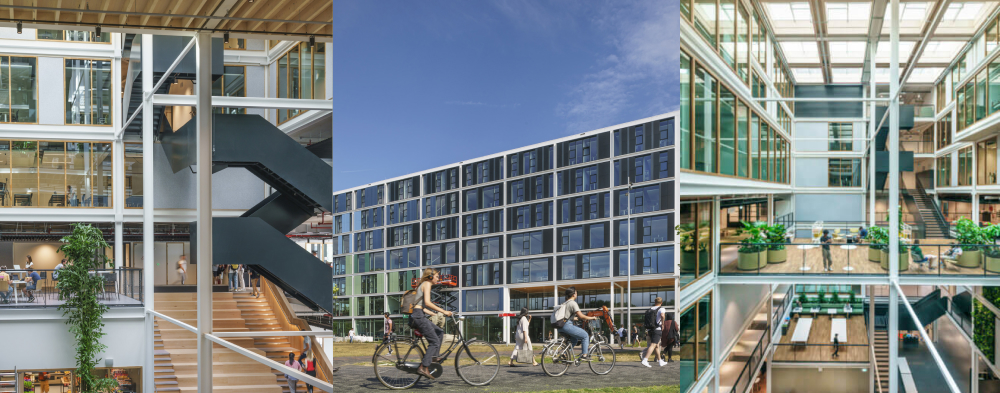
\includegraphics[width=0.45\textwidth,height=0.15\textwidth]{building_impressions.jpg}
    \caption{Impression photographs of the case study building}
    \label{fig:complexity}
\end{figure}

\subsubsection{Space usage}

The buildings's layout is strategically organized into different zones, each serving various functions, ranging from quiet individual work to spaces that allow for collaborative work. Lecture halls, learning rooms, and open learning spaces make up the two lower floors, with the upper four being primarily assigned to the university academic staff, meeting rooms, and external offices. The overarching interior theme in the design revolves around 'tech' and 'nature' aiming to cultivate a fresh, light, and warm comfortable ambiance. Lab42 is an example of a smart building or living lab where sensing devices are retrofitted throughout the building to automatically adjust lighting, temperature, and the focus of this research regulating air \cite{architects_lab42_2022}. This already provides a base of environmental data that can be used and extended for further analysis. Since most of the space within the building is designated as informal learning space and another large part of the building is designed as meeting rooms (see \hyperref[appendix:meetings]{Appendix \ref*{appendix:meetings}}), working areas these functions of focussed work and collaborative meetings can be heavily influenced by reduced cognitive performance as a result of poor indoor air quality.

\subsection{Questionnaire survey}
\label{sec:questionnaire}

To understand and collect occupants' subjective awareness and satisfaction of IAQ a structured survey was created to gather quantitative data within the building as a form of Post Occupancy Evaluation (POE) (see \hyperref[appendix:survey]{Appendix \ref*{appendix:survey}}).


\subsubsection{Questions}
The questions were based on two POE studies with a focus on indoor air quality \cite{silva_post-occupancy_2017, son_perceived_2023} and used standardized questions (e.g. Q-bank) and scales (e.g. Likert-scale). The survey consisted of a total of 9 questions (5 multiple choice, 3 Likert scales, 1 not mandatory open question) consisting of questions about:

\begin{enumerate}
  \item \textit{Activity and occupancy:} the rough location the occupant is within the building, how often the occupants use the building for various activities, and how they would describe the occupancy in their current space.
  \item \textit{Awareness and satisfaction:} how aware the occupant is of the current air quality in the space, how the occupant perceives the air quality in the current space, and how satisfied the occupant is with the air quality in the current space.
  \item \textit{Health and cognitive symptoms :} if the occupant experiences any health or cognitive symptoms based on the air quality in the current space.
\end{enumerate}


\subsubsection{Participants}
The survey was distributed via handouts with QR Codes using eligibility criteria based on demographic characteristics to occupants present at the informal learning spaces of the atrium, first floor, and second floor. There were no additional inclusion criteria besides the convenience sampling size of respondents being present in the case study building (sampling in context). Additionally, handouts were attached to the tables using stickers. All instances of participation were voluntary and conducted without remuneration. Distribution of the survey was open for submission from the 1st of March to the 31st of April 2024 which recorded X ($n$=X) responses in total of which after cleanup a total of X ($n$=X) responses were included in the final dataset. No personally identifiable information such as age and gender was collected during the survey and ethical considerations (e.g. consent forms) were taken into consideration. To improve the quality of the questionnaire on the initial version feedback was requested, after which the survey protocol was piloted, before distributing to participants (see \hyperref[appendix:experts]{Appendix \ref*{appendix:experts}}). 

\subsubsection{Data cleaning, preprocessing and analysis}
\label{sec:analysis}
After the distribution of the survey completed analysis of the collected data was performed in the form of data cleanup and exploratory data visualization. In Python (Jupyter Notebook format) \footnote{https://jupyter.org/} Libraries such as Numpy \footnote{https://pandas.pydata.org/} were used to clean the data (e.g. remove non-consenting users) and visualization libraries such as Seaborn \footnote{https://seaborn.pydata.org/} were used to create graphs and plots (e.g. boxplot the likert-scales) to get an overview of the collected data and gain insight into understanding the occupants.

\begin{figure*}[!t]
    \centering
    \begin{subfigure}[b]{0.23\textwidth}
        
\includegraphics[width=\textwidth]{placeholder.jpg}
        \caption{Placeholder caption}
        \label{fig:1}
    \end{subfigure}
    \hfill
    \begin{subfigure}[b]{0.23\textwidth}
        
\includegraphics[width=\textwidth]{placeholder.jpg}
        \caption{Placeholder caption}
        \label{fig:2}
    \end{subfigure}
    \hfill
    \begin{subfigure}[b]{0.5\textwidth}
        
\includegraphics[width=\textwidth, height=0.46\textwidth]{placeholder-two.jpg}
        \caption{Placeholder caption}
        \label{fig:3_4_combined}
    \end{subfigure}
    \caption{Impressions of the ideations and prototyping phase}
    \label{fig:full_width}
\end{figure*}

\subsection{Air Quality Monitoring}
\label{sec:monitoring}

To gather data about the current situation of air quality within the building and understand the current situation within the building in terms of air quality data we retrofitted IAQ monitors to two specific meeting rooms within the building (see \hyperref[appendix:floorplan]{Appendix \ref*{appendix:floorplan}}). This data collected was further used to inform and acted as a basis for the data input of the data physicalisation (see \hyperref[sec:prototype]{Section \ref*{sec:prototype}}).

\subsubsection{Technical set-up}

We deployed the monitors in meeting rooms occupants regularly use which allowed us to understand occupants' behavior and perception in real-world corporate settings as opposed to a controlled lab setting. We refer to them as the small room (room A) and the large room (room B). The small room is XX m2 and is commonly used for small-size meetings (seven seats), while the large room is XX m2 (fourteen seats), which is preferable for hosting larger-size meetings and seminars. Two commercially available indoor climate data loggers were installed using 3D printed mounting plates, an AirCheq Touch Aero \footnote{https://airteq.eu/producten/touch-aero/} in the smaller room and an Atal ATU-CT ClimaTrend \footnote{https://www.atal.nl/atu-ct-climatrend-binnenklimaat-datalogger} in the larger room. Both monitors use industry-standard (e.g. Senseirion and SenseAir) sensors to measure common pollutants and were mounted (e.g. between 80cm and 120cm from the ground) and calibrated (e.g. intervals, polling rates) as described by both manufacturer's installation manuals. The monitoring devices were installed from the 1st of March to the 31st of April 2024

\begin{table}[htbp]
    \centering
    \caption{Subset sample data of the IAQ monitors}
    \begin{tabular}{lccc}
        \toprule
        \textbf{Time} & \textbf{Humidity (\%)} & \textbf{VOCs (ppm)} & \textbf{CO2 (ppm)} \\
        \midrule
        08:00 & 40 & 0.05 & 500 \\
        09:00 & 42 & 0.06 & 520 \\
        10:00 & 45 & 0.07 & 550 \\
        \bottomrule
    \end{tabular}
    \label{tab:air-quality}
\end{table}

\subsubsection{Data logs}

The data gathered by the sensors provides insights into various standardized measurements related to common pollutants that affect IAQ such as molds and allergens (humidity), volatile organic compounds (VOC), and carbon dioxide (CO2) (see \hyperref[tab:air-quality]{Table \ref*{tab:air-quality}}, \hyperref[appendix:monitors]{Appendix \ref*{appendix:monitors}}). We cross-referenced the data logs with weekly schedules based on the internal booking systems of the rooms based on the timestamped data to align the values of the sensors from the data logs when meetings were scheduled. Data analysis is performed similarly as described in (see \hyperref[sec:analysis]{Section \ref*{sec:analysis}}). were data was cleaned to remove data from mainly non-opening hours and plotted and visualized to explore patterns in the data and cross-reference them with meeting times.


\subsection{Ideation and requirements}
\label{sec:ideation}

As a starting point for creating a physical representation of the air quality data we base our formative research on the growing interest in establishing theoretical and design foundations for \textit{data physicalisation} \cite{hornecker_design_2023, sauve_physecology_2022, bae_making_2022} on how to encode the properties and use a common design language \cite{ranasinghe_encoding_2023, sosa_data_2018} established by systematic reviews of data physicalization projects. The overall goal of the prototype is described in the following definition:

\AtBeginEnvironment{quote}{\setlength{\leftmargini}{10pt}}
\AtBeginEnvironment{quote}{\itshape}
\begin{quote}
a data-driven physical artifact whose geometry and material properties encode data that aims to augment a nearby audience’s understanding of data insights.
\end{quote}

Before prototyping the design solution we first describe the overall requirements and scope of the physicalization and case studies used for ideation. The final prototype is described based on the encoded variables and design dimensions found in the literature (see \hyperref[sec:prototype]{Section \ref*{sec:prototype}}).

\subsubsection{Concept requirements}

Based on this scope and the survey we describe the concept requirements ("r" for "requirements") of the design solution in further detail with six overarching requirements ranked based on the Moscow method:

\begin{enumerate}
    \renewcommand{\labelenumi}{R\arabic{enumi}:}
    \item \textbf{Visual Feedback:} The prototype must provide visual feedback through movement encoding environmental properties that represent air quality metrics, ensuring that users can easily interpret the information conveyed (must have).
    \item \textbf{Size and location:} The prototype must be designed to be installed within small to medium-sized rooms, with consideration for its dimensions and weight to ensure compatibility (must have).
    \item \textbf{Real-Time Data Integration:} The prototype should integrate real-time data from air quality monitors to dynamically adjust its behavior (should have).
    \item \textbf{Interactive sensing:} The prototype should be interactive in which occupants can interact with the prototype by walking near it providing a tactile experience (should have).
    \item \textbf{Material durability:} The prototype could use natural materials and be durable and resistant to environmental factors such as humidity and temperature fluctuations (could have).
    \item \textbf{Aesthetic Integration:} The prototype could seamlessly integrate with its surrounding environment, complementing interior design aesthetics, architectural features, and layouts of the room to enhance the overall ambiance (could have).
\end{enumerate}

\subsubsection{Concept models}

For the concept models, two existing datasets of academic and non-academic case studies were used as comparative studies, desk research, and as a starting point for ideation. First was the DataPhys gallery \footnote{http://dataphys.org/list/gallery/}, a collection of 372 entries classified as data physicalizations. The second was a combination of three state-of-the-art papers with systematic reviews of physicalization with combined examples of around 132 entries classified as data physicalization of which both academic and non-academic samples \cite{sauve_physecology_2022, anhalt_university_germany_design_2022, ranasinghe_encoding_2023}. Out of these, seven ($f$=7) samples of academic were selected for further review based on the similarity with the before described requirements of which three ($f$=3) samples with a focus on the environmental property of air, but not necessarily air quality within indoor environments (see \hyperref[appendix:academic]{Appendix \ref*{appendix:academic}}). Additionally, fifteen ($f$=15) samples of non-academic case studies were reviewed after desk research which included work and prototypes from design studios and independent creators that informed the ideation phase (see \hyperref[appendix:nonacademic]{Appendix \ref*{appendix:nonacademic}}).

\subsubsection{Concept diagrams}

Based on the user requirements and ideation and concepting from the Communication and Multimedia Design (CMD) Methods Pack \footnote{https://cmdmethods.nl/} and Design Method Toolkit \footnote{https://toolkits.dss.cloud/design/} by the Digital Society School (DSS) three low fidelity (lo-fi) concepts were further elaborated (see \hyperref[fig:3_4_combined]{Figure \ref*{fig:3_4_combined}}) in order to choose one to develop in high fidelity (hi-fi) for the user studies and evaluation. 


\begin{enumerate}
  \item \textbf{Concept-1: Desk Planter (Aspen)}
      A desk planter or tree in the corner of the room with soil in it.Follows the organic growth of a 'seed' of a flower or tree from seed to sprouts to full flower. The better the air quality the more or faster the plant grows. The movement of the leaves can indicate the wind.

  \item \textbf{Concept-2: Hanging Sculpture (Bluebird)}
      A hanging planter-type set-up with strings that 'grow' from the ceiling. Fresh air moves the strings. People can walk by, and feel the material (e.g. humidity). Allows most interactivity. Taking inspiration from kinetic sculptures and hanging/floating sculptures.

  \item \textbf{Concept-3: Wall Kinetic (Crocus)}
      A moss-like structure on the wall with flower bulbs embedded. The flowers 'open up' based on better fresh air. Taking inspiration from kinetic sculptures.
\end{enumerate}


Concept selection was based on weighted physicalization criteria from the literature, a Harris profile for the lo-fi concepts, and four expert reviews ($n$=2 internal experts involved in the project, $n$=2 external experts not involved in the project) feedback (see \hyperref[appendix:profile]{Appendix \ref*{appendix:profile}}, \hyperref[appendix:expert]{Appendix \ref*{appendix:expert}}). Also technical limitations of the provided hardware (e.g. real-time data output of monitors, cost of hardware, availability of electronic components,) and limitations in the technical set-up of the building (e.g. space in the meeting rooms, not allowed to alter furniture) were considered as heuristic evaluation. Based on the aggregation of these criteria the \textit{Bluebird} concept was chosen to be further developed into a high-fidelity prototype (see \hyperref[fig:bluebird]{Figure \ref*{fig:bluebird}}, \hyperref[appendix:prototype]{Appendix \ref*{appendix:prototype}}).

\subsection{Evaluation}
\label{sec:evaluation}

The prototype was evaluated as summative research using common performance-related criteria that are widely used in HCI/Information Visualisation \cite{ranasinghe_encoding_2023} and Grounded Theory studies \cite{chun_tie_grounded_2019}. We employed a field-based evaluation approach with accompanying methods based on the Human-centered Design Kit by Ideo \footnote{https://www.designkit.org/methods.html} and Delft Design Guide from the Delft University of Technology (TU) \footnote{https://www.bispublishers.com/delft-design-guide-revised.html}. For evaluation criteria, we used the intentions and evaluating interview methodology described in the data physicalization design vocabulary \cite{jansen_evaluating_2013,ranasinghe_encoding_2023} as a baseline for evaluating the efficiency, and memorability using in-person evaluation sessions. To measure the overall effectiveness and usability of the physicalization we based and adopted questionnaires of the Technology Acceptance Model (TAM) and System usability scale (SUS) to gather insight into perceived usefulness, attitude towards using, and system usability scale \cite{davis_perceived_1989, brooke_sus_1996}. 

\subsubsection{Hypothesis elicitation}

Based on the research question and creation of the prototype three hypotheses ("h" for "hypothesis") were formulated to evaluate as an observational study:

\begin{enumerate}
    \renewcommand{\labelenumi}{H\arabic{enumi}:}
    \item \textbf{Understanding:} users will exhibit a clear comprehension of the physicalization's representation of IAQ data, as well as an understanding of its intended function and impact
    \item \textbf{Self-reflection:} users exposure to real-time IAQ data visualizations through the prototype will prompt users to reflect and will lead to increased awareness.
    \item \textbf{Effectiveness:} users acceptance and satisfaction with the IAQ physicalization will be positively correlated with perceived usefulness, attitude towards use, and system usability.
\end{enumerate}

\subsubsection{Participant sampling}

The sample size of evaluation interviews was x ($n$=X) and accepted because the study findings reached theoretical saturation, new interviews did not yield new insights after the first x interviews and led to repetitive data \cite{steph_menken_introduction_2016}. Participants were gathered through purposive sampling and were not involved in the development of the prototype. Respondents had to meet the inclusion criteria ("c" for "criteria") that needed to be checked before the interviews: 

\begin{enumerate}
    \renewcommand{\labelenumi}{C\arabic{enumi}:}
    \item The participant needed to use a meeting room with the building a minimum of once a week
    \item The participant needed to work within the case study week a minimum of 3 days per week
\end{enumerate}

This resulted in a sample of x male, x female, consisting of various roles; from researchers from different labs, PhD candidates working at the labs to private company employees encompassing a range of ages ($min$=x, $max$=x, $mdn$=x) and education levels of which x ($f$=x) participants were acquired through snowball sampling. Participants used the meetings rooms on average x ($min$=x, $max$=x, $mdn$=X) a week and worked within the lab42 building x ($min$=x, $max$=x, $mdn$=X) a week. The evaluation session where held between May 1st to 31st of May 2024

\subsubsection{Evaluation interviews}

Within the meeting-room lab set-up in the presence of the developed prototyped pre-arranged, semi-structured individual qualitative interviews were conducted with open-ended and nonleading questions with additional in-depth questions (follow-up probing strategy) on topics emerging from the dialogue (see \hyperref[appendix:evaluation]{Appendix \ref*{appendix:evaluation}}). To improve the quality of the interviews (and evaluation session in general) on the initial version feedback was requested, after which the interview protocol was piloted, before continuing with participants (see \hyperref[appendix:experts]{Appendix \ref*{appendix:experts}}). The goal was to gather first impressions and gain insight into how occupants understand the communicated data factors of the prototype.

\subsubsection{Participant observation (usability testing)}

After the explorative questions participants were encouraged to in more detail view the prototype and interact with it as a field trial stating anything they noticed (encouraging probing strategy). Participants' behavior was observed within prolonged engagement in the meeting rooms and participants were encouraged to think aloud when viewing and interacting with the prototype (see \hyperref[appendix:usability]{Appendix \ref*{appendix:usability}}). Informal leading questions were asked about improvements, design optimization, and visual changes. In this manner, insights into particular interaction elements were acquired without the explicit involvement of HCI specialists. The goal was to test the usability of the prototype, study occupants and their behavior in a natural setting, and gather insight into the self-reflective properties of the prototype. 

\subsubsection{Prototype effectiveness}

After the interviews and observations, the participants were asked to fill in a digital online with structured pre-defined questions form rating several properties of the prototype for their effectiveness (see \hyperref[appendix:effectiveness]{Appendix \ref*{appendix:effectiveness}}). The goal was to gather quantitative measurements about the usability and effectiveness of the prototype.

\subsubsection{Transcription and coding}
All interviews were anonymized and conducted in-person on-site and audio recorded with permission of the participants. The recordings were then verbatim transcribed using the built-in Microsoft 365 transcription tool \footnote{https://www.microsoft.com/nl-nl/microsoft-365} to avoid bias while note-taking. The transcribed interviews as textual data were processed via Atlas.ti \footnote{https://atlasti.com/} for qualitative coding.

\begin{figure*}[b]
    \centering
        \begin{subfigure}[b]{0.45\textwidth}
        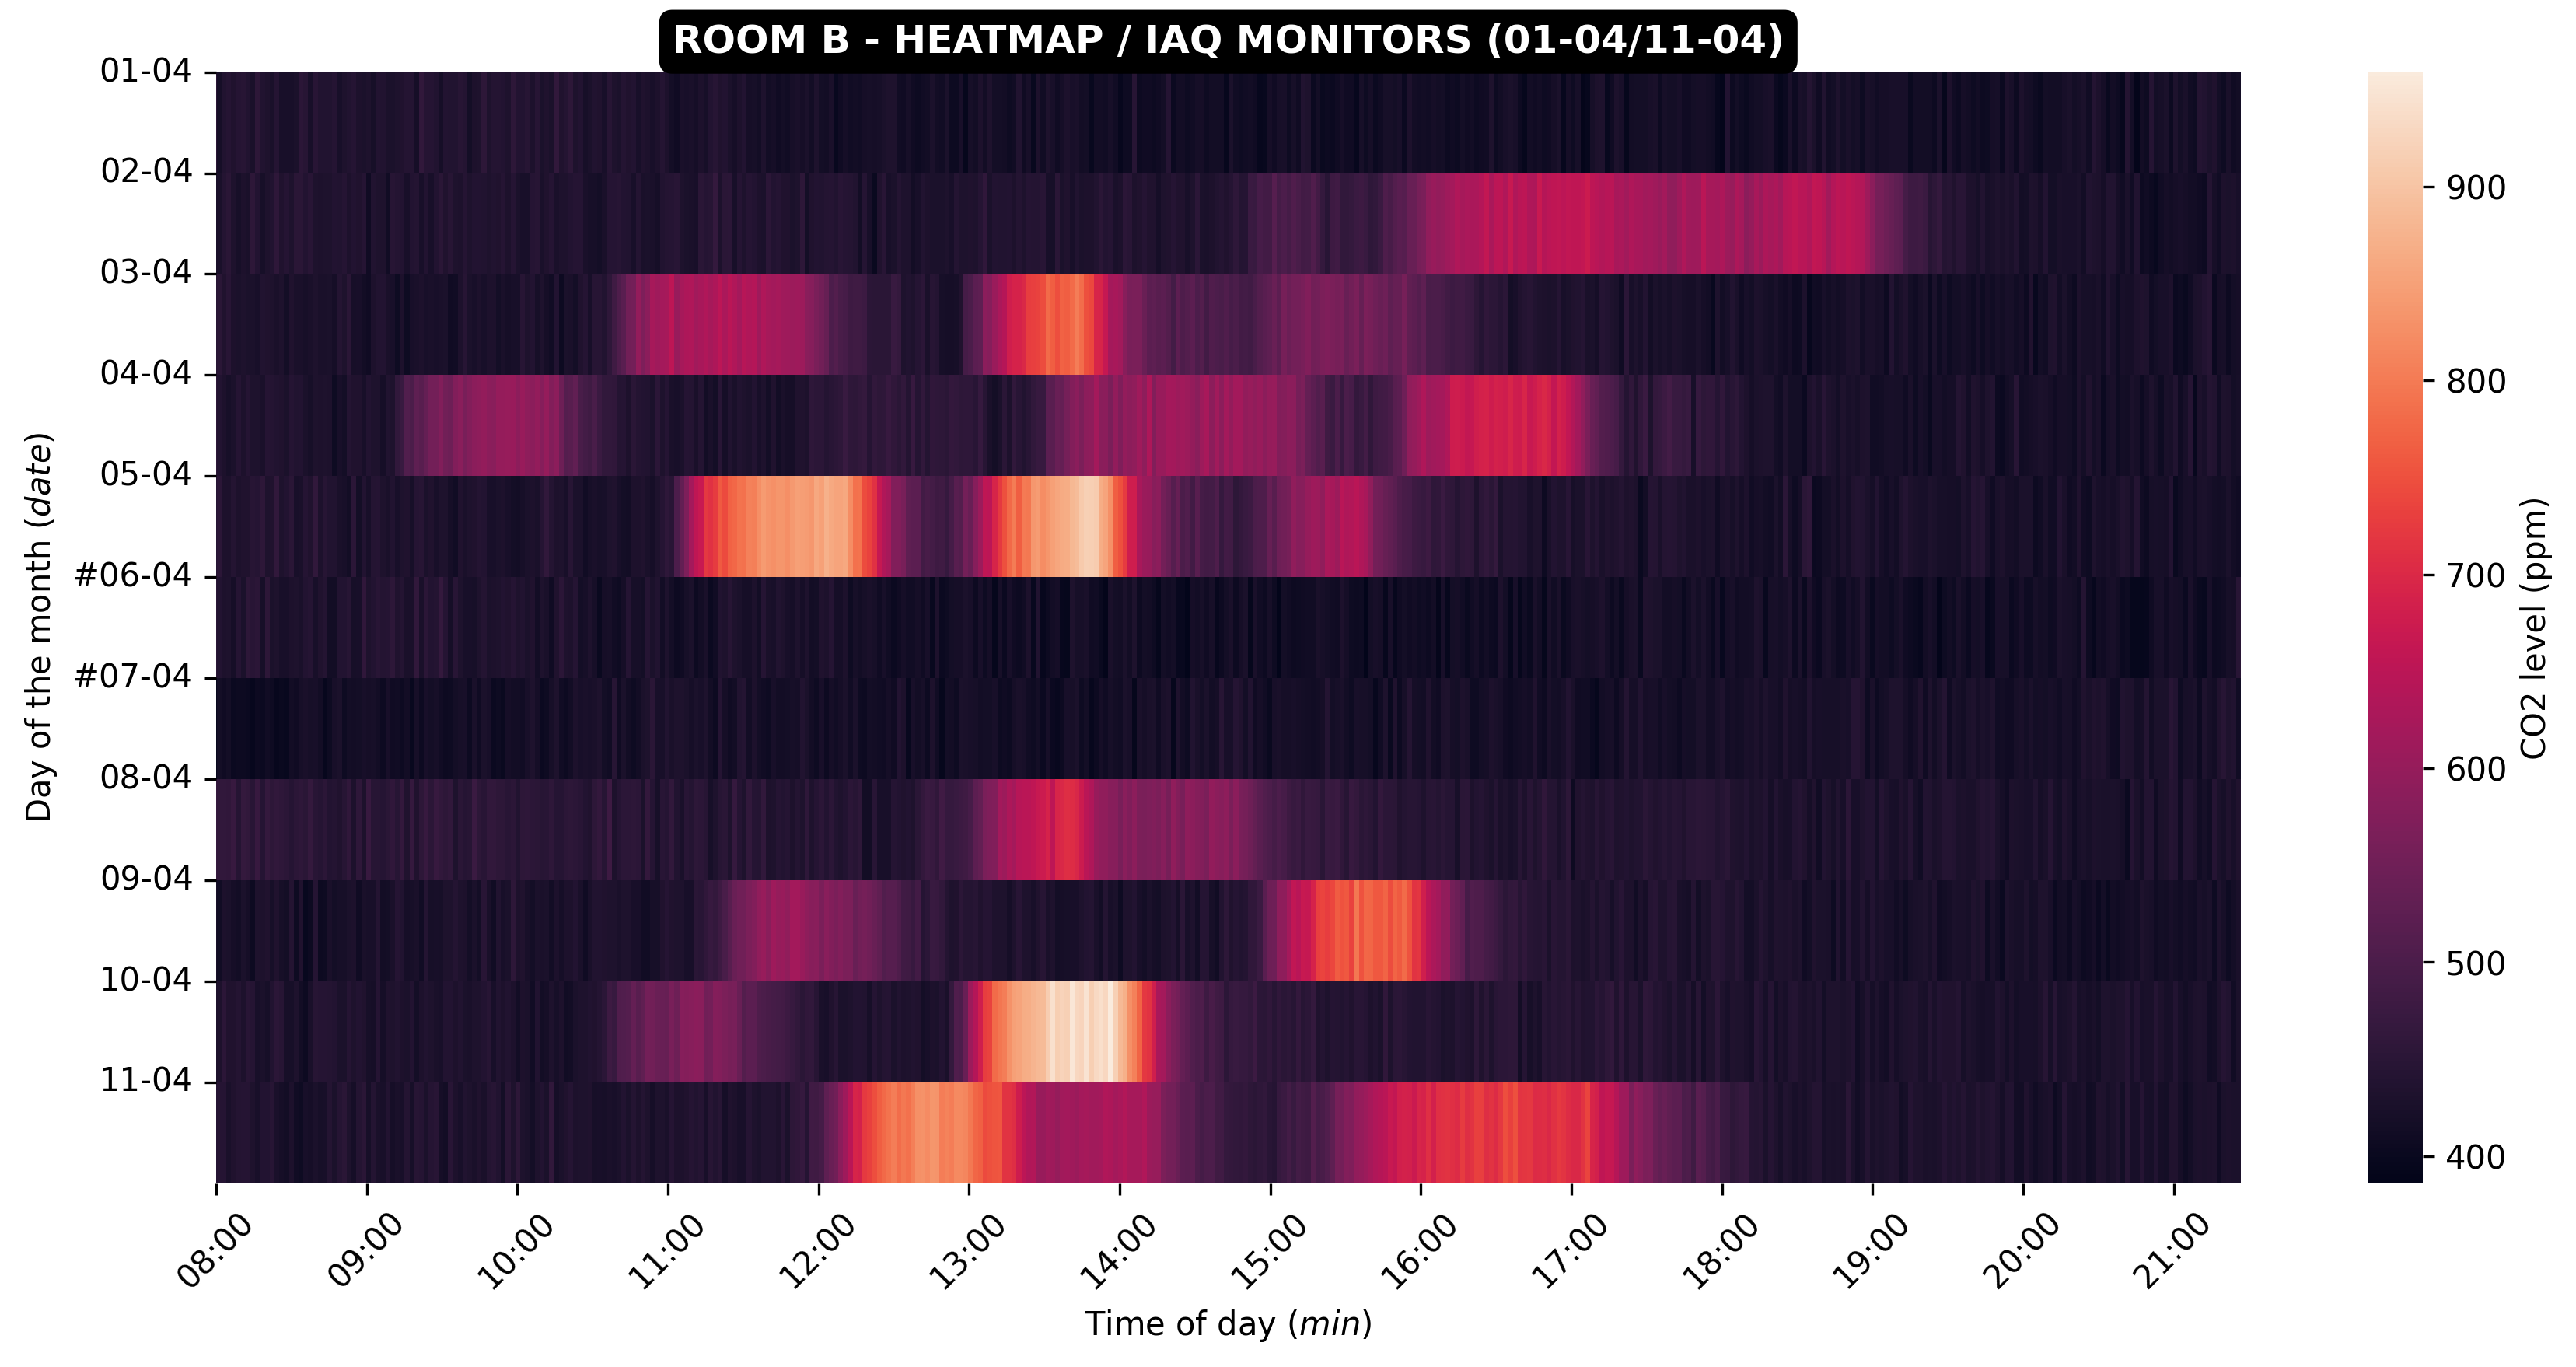
\includegraphics[width=\textwidth]{room-b-monitor-heatmap.png}
        \caption{Heatmap of Room B with ten days of data collection}
        \label{fig:3_4_combined}
    \end{subfigure}
    \begin{subfigure}[b]{0.5\textwidth}
        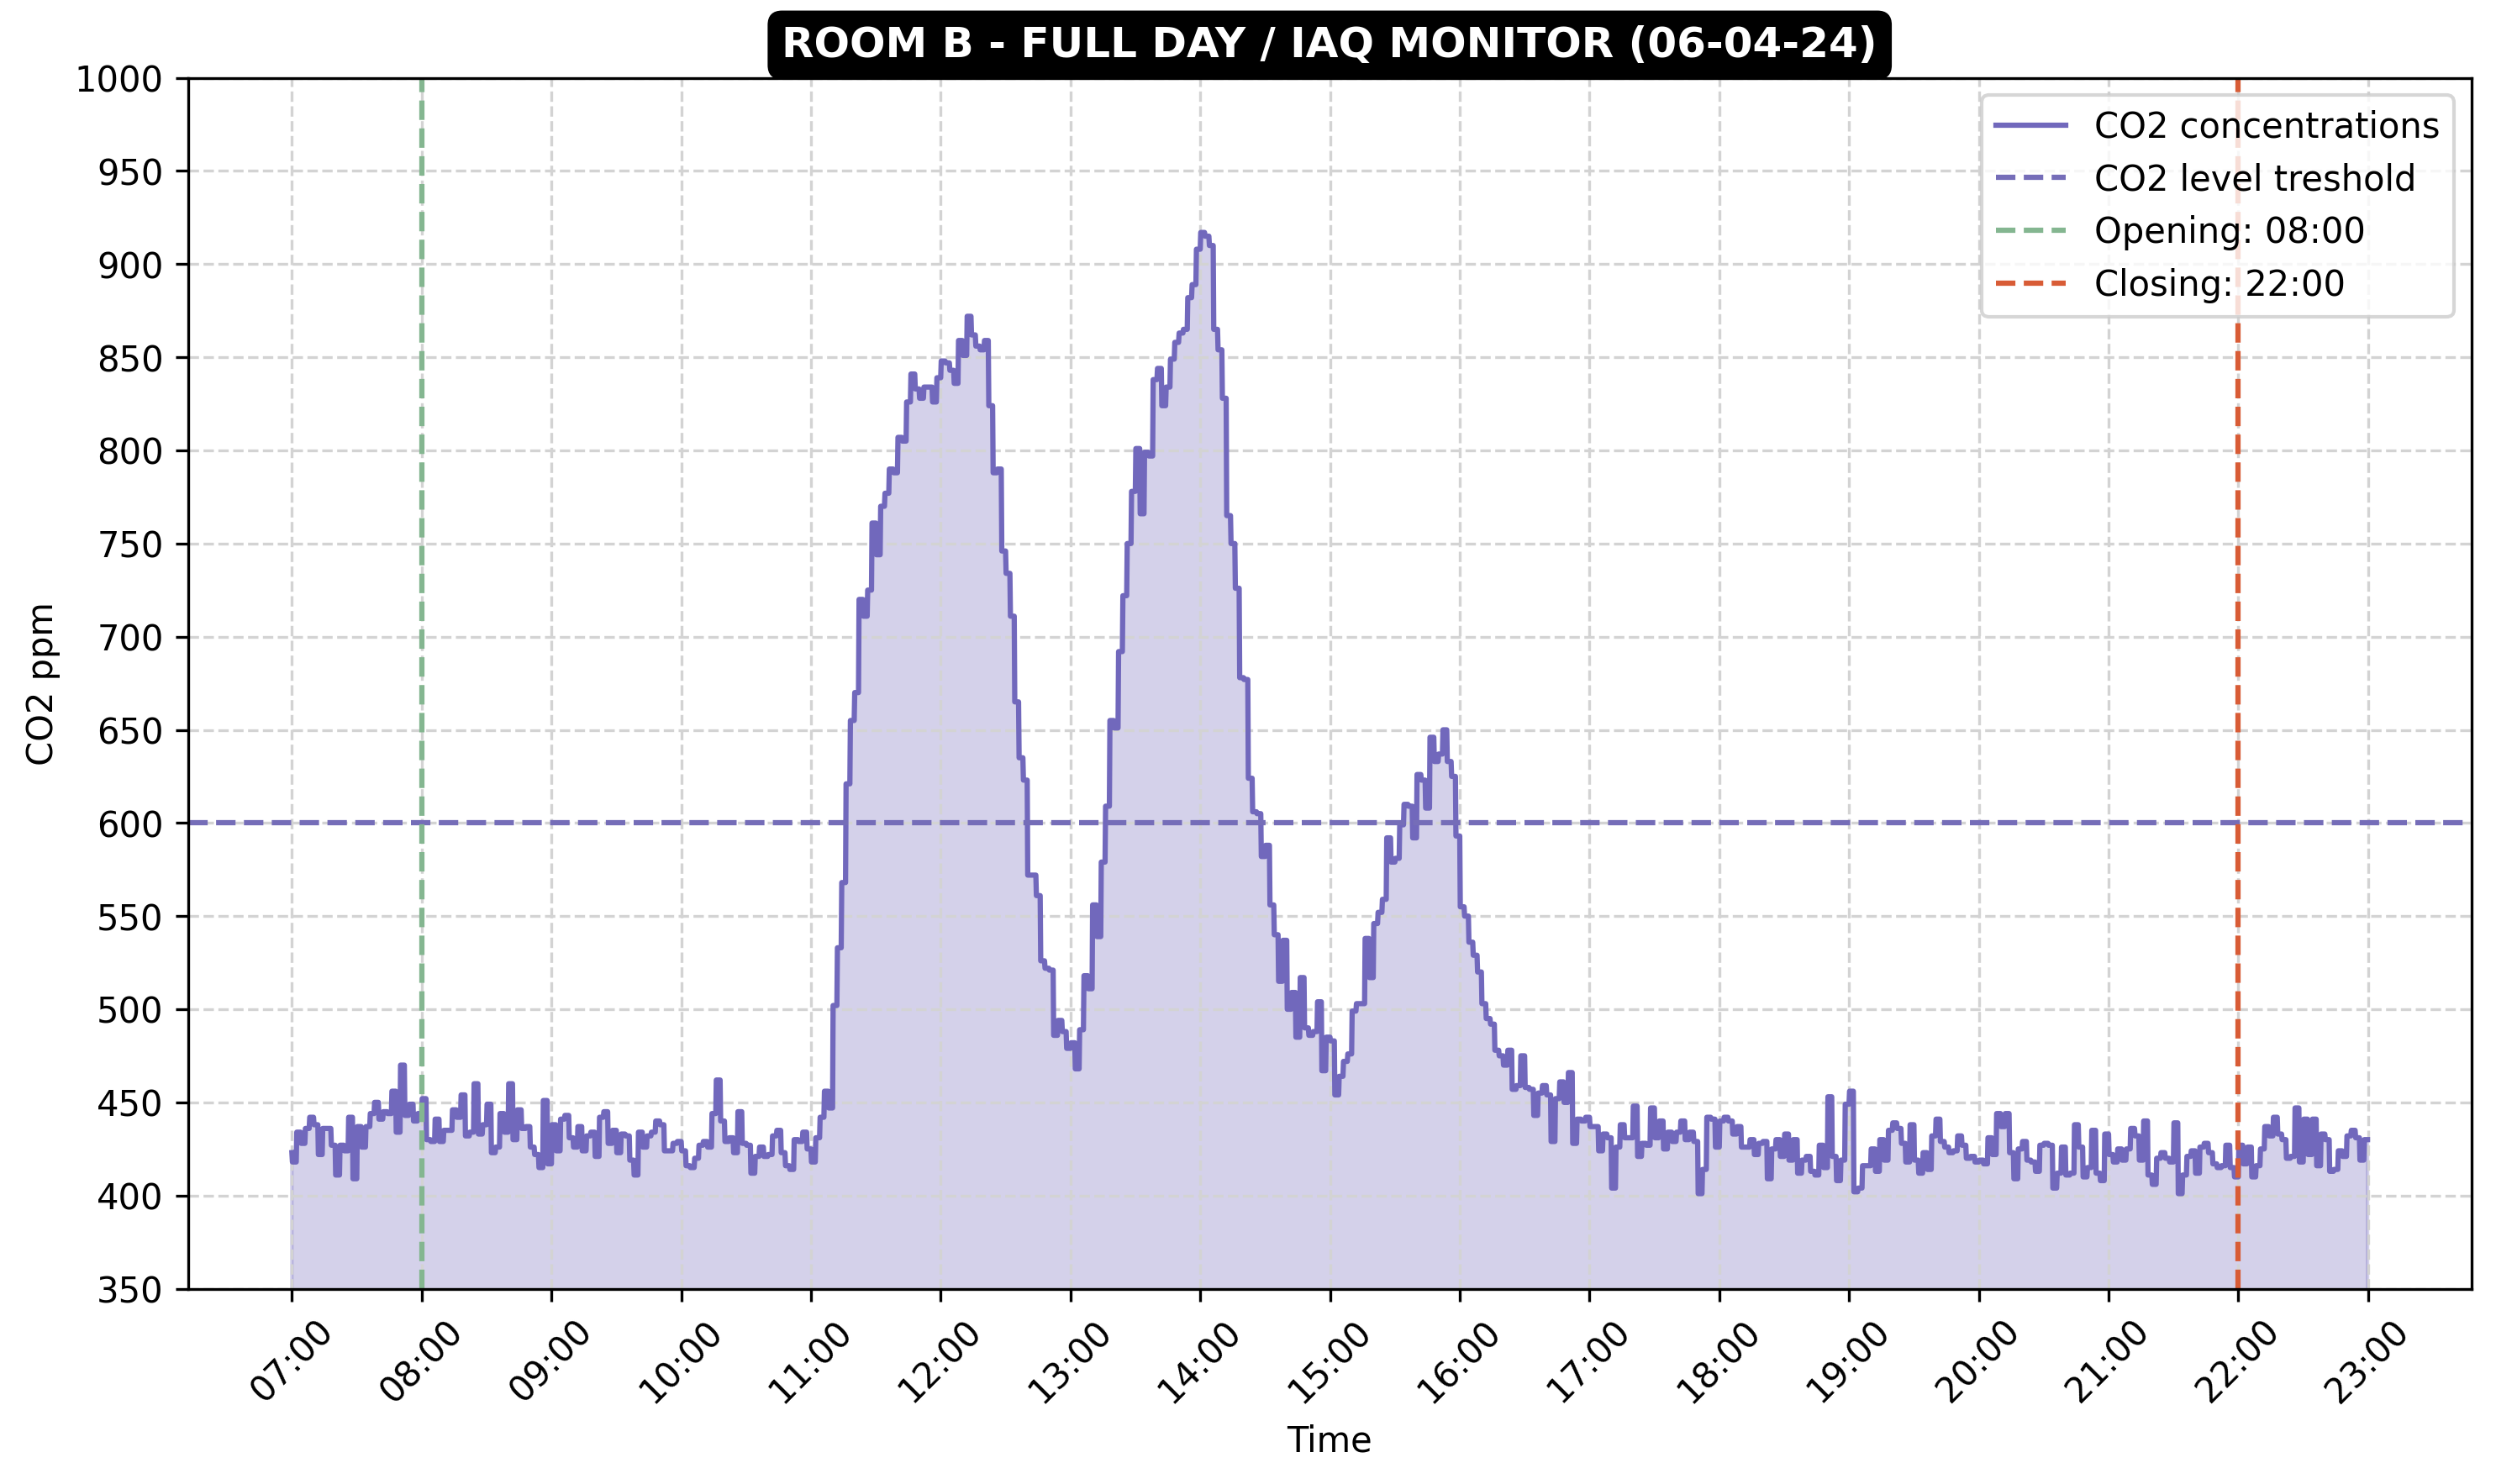
\includegraphics[width=\textwidth]{room-b-monitor-meeting-spike-day.png}
        \caption{Lineplot of Room B with a single day of meetings}
        \label{fig:1}
    \end{subfigure}
    \hfill
    \caption{Plots of the IAQ monitor data logs CO2 concentrations within the meeting rooms}
    \label{fig:full_width}
\end{figure*}